\section{Description And Methodology}

\subsection{Initial Setup}
To begin with, peripherals such as buttons, LEDs, DAC, and timers needed to be configured. As C programs can control hardware directly, one only needs to use pointers to refer to memory-mapped I/O registers. A lot of these were provided in the efm32gg.h-file where many of the registers were defined with macros by using volatile $uint32\_t$ pointer variables, so in the initial setup it was simply a matter of dereferencing these and writing the appropriate values.

\subsubsection{Interrupt handlers}
The procedure for setting up interrupt handlers will vary depending on the hardware used. To enable interrupt generation and interrupt handling for the appropriate exception handlers, the proper value had to be written to the ISER0-register, which was done in the setupNVIC()-function in the ex2.c-file. The hexadecimal value 0x1802 written to the ISER0-register corresponds to writing bit 1, 11, and 12 in the register, which are the appropriate bits for enabling interrupts for the mentioned exception handlers.
	The code for the exception vectors was already filled out in the startup code, so all that needed to be done to use the exception handlers was to write a function in the form $\_\_attribute\_\_$ ((interrupt)), as this tells the compiler that this is a function used for exception handling.

\subsubsection{Timers}
There are several hardware timers that can be used, depending on the purpose (calculation-intensive operations, low energy demands, etc...). The timers have the advantage of being able to produce interrupts at periodic intervals. These make them ideal when working with sounds where the creations of sound waves depends consistent oscillations. 

The timer was configured to be set to a specific frequency through the use of the TOP register. The interrupt frequency was determined by dividing the timer clock frequency by the amount of interrupts required. The TOP register specifies the number of clock cycles between each interrupt

\subsubsection{Digital to analog converter (DAC)}
The DAC is a component that converts a digital value to an analog signals. The DAC on the EFM32GG has two channels, each with a 12-bit data register. The EFM32GG has several modes of writing to the DAC, with continous mode being the simplest one. How to set up the DAC in this mode was well specified in the compendium, and was implemented in the setupDAC()-function in the dac.c-file. Writing 0x50010 to the $DAC0\_CTRL$ register enables DAC-output in continous mode. As we learned later, altering  this value to, for instance, 0x50014, will enable the DAC-output to sample/hold mode instead of continous mode, which has other advantages. This will be explained in greater detail in the Energy Optimization section. 
	Bit 16, 17, and 18 of said control register decided prescaling value (PRESC) in such a way that the DAC clock frequency is set by:

\begin{center}

$f_{DAC\_CLK} = \frac{f_{HFPERCLK}}{2^{PRESC}}$

\end{center}

Since PRESC can be any value between 0 and 7, the fraction part of the equation can be between 1 and 128. In our case, we used a prescaling value of $101_2$, or $5_{10}$. With this value, and a high peripheral clock frequency of 14 MHz, the DAC clock frequency was set to:

\begin{center}

$f_{DAC\_CLK} = \frac{f_{HFPERCLK}}{2^{5}} = \frac{14000000 Hz}{32} = 437.5 KHz $

\end{center}

\subsection{Sound Wave Synthesis}

Sound is created through sound waves, which are created by oscillations, or a consistent, repeating signal. These oscillations can be used to create waves at various frequencies, as sound are the properties of the waves generated, with respect to the frequency, amplitude, and period. The frequency determines the tone of the sound, the amplitude the strength, and the period the duration of the sound.

There are various approaches for generating these sound waves. The different wave types have slightly different properties in regard to sound. For instance, we have the sine wave, sawtooth wave, triangle wave and the square wave. These waves have different sound characteristics. For instance, an ideal square wave will make instantaneous transitions between high and low levels, whereas an ideal sawtooth wave will "climb" to the highest amplitude level, then instantaneously drop down to its lowest level and repeat. These two waves are illustrated in the figures below.

\begin{figure}[H]
  \centering
  % Trim er [left bottom right top]
  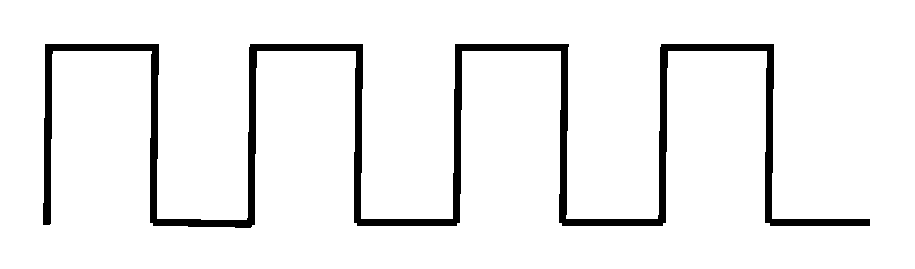
\includegraphics[clip, trim=0cm 0cm 0cm 0cm, width=4cm]{fig/square_wave.pdf}
  \caption{Square wave}
\end{figure}

\begin{figure}[H]
  \centering
  % Trim er [left bottom right top]
  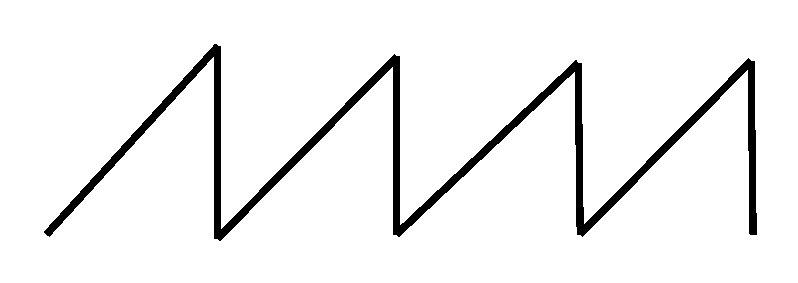
\includegraphics[clip, trim=0cm 0cm 0cm 0cm, width=4cm]{fig/sawtooth.pdf}
  \caption{Sawtooth wave}
\end{figure}


The waves shown above are the two types we have created and tested in this assignment. 

The different notes were defined as macros A through O in the sounds.h file, each as a frequency between 200 and 3000 Hz. These were mainly used for creating specific sound effects, which will be described in further detail in the User Control section.
	
In order to play tones for a specified amount of time, we defined a struct in the sounds.h-file with a note and time field, where note would be specified in Hz, and time in milliseconds. Each of the melodies in the melodies.h-file were made as arrays of said structs. The playSong()-function would then be responsible for playing these melodies by continously calling on the testNotes()-function and iterating through the array. A square waveform with a peak-to-peak amplitude of 4000 was used, as this generated a comfortable sound level. The square wave was created by calculating discrete samples based on tone and oscillator frequency, where the oscillator frequency divided by the tone frequency decided how often the values to the DAC should alternate, thereby producing an approximation of the note. This was also tested with an implementation of the sawtooth waveform, which was implemented as a linear function where the rising slope was calculated by dividing the peak amplitude by the number of samples per wave. The value written to both DAC-channels would then be calculated by multiplying the slope with the duration variable, which would be incremented until it was equal to or greater than the sampling value, much in the same fashion as in the square waveform implementation.
	Using the square waveform instead was prefered in the end due to the overly 'sharp' sound of the sawtooth waveform.

\subsection{Sound Sampling}

Sound can also be generated through pre computed samples. With this approach, the sound waves are generated on some other platform. The samples produced are approximations of already existing sound samples. The samples are modified slightly to fit the microcontroller. Due to size limitations on the board, 8 bit samples at 8000Hz were generated. This decreased the sound quality, but allowed us to be able to play songs with greater length. In the first approach we generated samples with a sample frequency of 48000Hz. This sample rate produced sounds with relatively high sound quality, but required a substantial amount of storage.

The sound samples were generated with the use of Audacity and Switch. These programs were used to change the size of the samples and adjust the sample rate. The samples were then further extracted from the .wav files, and extracted into an array consisting of 8-bit chars. The sample array could then be then statically linked with the code. However, the relatively low sample rate required some changes in the code. Note that the sound synthesiser used a sample rate of 48000 instead. In order to be able to play the samples at 8000Hz we had to adjust the sample frequency when playing the precomputed samples. This was achieved by simply changing TOP register of the timer. By adjusting this register we were able to change the interrupt frequency, and thereby changing the sample frequency, so that each sample could simply be played at each interrupt.  



  














\subsection{Energy Optimization}
The EFM32GG microcontroller has a rich set of features regarding improving energy efficiency, where the main focus is turning of components that are not in use, or tuning their performance. We have utilised many of these techniques to improve the power consumption of the program, where our main goal has been to try to exploit the various energy levels that the microcontroller has to offer, preferably being able to achieve EM3 and turn of every component not in use. 

Various techniques were employed to reach this goal. As it turned out, achieving deep sleep and sleep on exit proved to be more complicated than first imagined. During deep sleep mode the high frequency oscillator was turned off. This oscillator was used to clock both the DAC and the timer. When entering EM3 this produced some unexpected bugs. On entering EM2 the program started to behave non-deterministic. As it turned out, both the DAC and the timer was clocked by the high frequency oscillator. This directly affected the interrupts produced by the timer. This problem was solved by introducing the low energy timer. This timer is able to run as low as EM2 and EM3 depending on the oscillator used. For producing sound, the 32.768 KHz oscillator was used. This timer replaced the old timer, and only caused some minor changes to made in the already existing code. In particular, the frequency used to generated was changed to accommodate the new oscillator frequency. Instead of  using a sample rate of 48000, the new oscillator was able to produce 32768 interrupts every second. This implied a maximum sample rate of 32768. Fortunately, our tone frequencies were sufficiently low to accommodate this change in sample frequency. However, while this reduced the energy consumption, there were still some problems with the DAC, as entering a lower energy mode caused the DAC to continue producing static sound. As it turns out, configuring the DAC with continuous mode will not be able to maintain the voltage levels when entering deep sleep. This caused the voltage levels to fluctuate, and create a static background sound. Fortunately, the DAC also support another mode, sample/hold mode. During sample/hold mode, the DAC core converts on a triggered conversion and then holds the output in a sample/hold element. When not converting, the DAC is turned of between samples, which reduces the power consumption. The sample/hold element will hold the element for a certain time without needing a refresh conversion\cite{EFM32GG-rm}. Switching to this mode not only fixed our bug, but also further decreased the energy consumption. This change from continuous mode to sample/hold mode is achieved by changing the value written to the $DAC0\_CTRL$ register from 0x50010 to 0x50014. 

These techniques allow the code to enter deep sleep mode, and also allow utilisation of sleep on exit. This is was accomplished by writing the value 6 to the SCR register setting the deep sleep and deep sleep on exit bit. Entering EM3 is then achieved by calling the WFI instruction.

These techniques combined proved to be very beneficial regarding the energy efficiency. However, even further improvements could be made. While the high frequency oscillator was turned off during deep sleep, the energy timer would still consume power. To allow the program achieve even better decrease in power consumption, we implemented functions that could enable/disable these components. Said components were only enabled when needed, and disabled during idle mode.



\subsection{User Control}
In order to let a user be able to interact with our setup, the buttons on the gamepad were configured so that different sounds would play when one of them were pressed. Each button was configured to play one specified sound or melody. This was done by reading the value of the $GPIO\_PC\_DIN$ register, and writing this value to a function $play\_melodies(int)$ that would take the $GPIO\_PC\_DIN$ value as an input parameter and play the corresponding melody. One of the challenges in this was to get the DAC to output the entire melody, and not just for the duration in which a button was pressed. To solve this, a pointer variable was used to point to the correct sample array and let the timer run for the entire length of the array in order to play the whole melody. An alternative approach was to declare a global variable and set it to the value of the $GPIO\_PC\_DIN$ register in each of the GPIO-handlers, and use a switch-statement in the low-energy timer function to play the corresponding melody, but the former approach was prefered due to its energy efficiency advantages.

Our setup was as follows:

\begin{table}[ht]
\caption{Buttons and corresponding melodies}
% title of Table
\centering
% used for centering table
\begin{tabular}{c c}
% centered columns (4 columns)
\hline
\hline %inserts double horizontal lines
Button & Melody \\ [0.5ex]
% inserts table
%heading
\hline
SW1 & Mario \\
SW2 & Shoot \\
SW3 & Hit dealt \\
SW4 & Hit received \\
SW5 & Battlefield intro \\
SW6-SW8 & Simple *beep*-noises \\
% [1ex] adds vertical space
\hline
%inserts single line%
\end{tabular}
\label{table:nonlin}
% is used to refer this table in the text
\end{table}